\documentclass[a4paper,11pt]{article}
\usepackage{amsmath,amsthm,amsfonts,amssymb,amscd,amstext,vmargin,graphics,graphicx,tabularx,multicol} 
\usepackage[francais]{babel}
\usepackage[utf8]{inputenc}  
\usepackage[T1]{fontenc} 
\usepackage{pstricks-add,tikz,tkz-tab,variations}
\usepackage[autolanguage,np]{numprint} 

\setmarginsrb{1.5cm}{0.5cm}{1cm}{0.5cm}{0cm}{0cm}{0cm}{0cm} %Gauche, haut, droite, haut
\newcounter{numexo}
\newcommand{\exo}[1]{\stepcounter{numexo}\noindent{\bf Exercice~\thenumexo} : \marginpar{\hfill /#1}}
\reversemarginpar


\newcounter{enumtabi}
\newcounter{enumtaba}
\newcommand{\q}{\stepcounter{enumtabi} \theenumtabi.  }
\newcommand{\qa}{\stepcounter{enumtaba} (\alph{enumtaba}) }
\newcommand{\initq}{\setcounter{enumtabi}{0}}
\newcommand{\initqa}{\setcounter{enumtaba}{0}}

\newcommand{\be}{\begin{enumerate}}
\newcommand{\ee}{\end{enumerate}}
\newcommand{\bi}{\begin{itemize}}
\newcommand{\ei}{\end{itemize}}
\newcommand{\bp}{\begin{pspicture*}}
\newcommand{\ep}{\end{pspicture*}}
\newcommand{\bt}{\begin{tabular}}
\newcommand{\et}{\end{tabular}}
\renewcommand{\tabularxcolumn}[1]{>{\centering}m{#1}} %(colonne m{} centrée, au lieu de p par défault) 
\newcommand{\tnl}{\tabularnewline}

\newcommand{\trait}{\noindent \rule{\linewidth}{0.2mm}}
\newcommand{\hs}[1]{\hspace{#1}}
\newcommand{\vs}[1]{\vspace{#1}}

\newcommand{\N}{\mathbb{N}}
\newcommand{\Z}{\mathbb{Z}}
\newcommand{\R}{\mathbb{R}}
\newcommand{\C}{\mathbb{C}}
\newcommand{\Dcal}{\mathcal{D}}
\newcommand{\Ccal}{\mathcal{C}}
\newcommand{\mc}{\mathcal}

\newcommand{\vect}[1]{\overrightarrow{#1}}
\newcommand{\ds}{\displaystyle}
\newcommand{\eq}{\quad \Leftrightarrow \quad}
\newcommand{\vecti}{\vec{\imath}}
\newcommand{\vectj}{\vec{\jmath}}
\newcommand{\Oij}{(O;\vec{\imath}, \vec{\jmath})}
\newcommand{\OIJ}{(O;I,J)}


\newcommand{\bmul}[1]{\begin{multicols}{#1}}
\newcommand{\emul}{\end{multicols}}

\newcommand{\reponse}[1][1]{%
\multido{}{#1}{\makebox[\linewidth]{\rule[0pt]{0pt}{20pt}\dotfill}
}}

\newcommand{\titre}[5] 
% #1: titre #2: haut gauche #3: bas gauche #4: haut droite #5: bas droite
{
\noindent #2 \hfill #4 \\
#3 \hfill #5

\vspace{-1.6cm}

\begin{center}\rule{6cm}{0.5mm}\end{center}
\vspace{0.2cm}
\begin{center}{\large{\textbf{#1}}}\end{center}
\begin{center}\rule{6cm}{0.5mm}\end{center}
}



\begin{document}
\pagestyle{empty}
\titre{Contrôle sur les 3 premiers chapitres}{Nom :}{Prénom :}{Classe}{Date}



\exo{5} \\

\q Relier chaque phrase à l'expression qui lui correspond (\textbf{sur le sujet})

\begin{multicols}{2}

\bi
\item La somme de 9 et du quotient de 7 par 2.\\

\item Le produit de 7 par la somme 9 et de 2.\\

\item Le quotient de 9 par la somme 7 et de 2.\\

\item La somme de 9 et du produit de 7 par 2.\\

\item Le quotient d'une somme par 2.
\ei

\hfill
\columnbreak
\hfill

\bi
\item $A= 9 + 7 \times 5$\\

\item $ B= 7 \times (9 +2)$\\

\item $ C=9 + \dfrac{7}{2}$\\

\item $D= \dfrac{9+7}{2}$\\

\item $E= \dfrac{9}{7+2}$
\ei 

\end{multicols}

\q Calculer les expressions A, B, C, D et E.


\vspace*{0.6cm}

\exo{2}(\textbf{Sur le sujet})

Chacune des expressions suivantes est fausse. Placer, dans chaque cas, des parenthèses aux bons endroits pour rendre l'égalité vraie.\\


\qa 2 $\times$ 5 + 2 = 14\\

\qa	1 + 3 + 2 $\times$ 6 = 31\\

\qa	1 + 2 $\times$ 5 + 3 $\times$ 10 - 4 = 33

\vspace*{0.6cm}

\exo{4}\\

Calculer les expressions suivantes en respectant les priorités (on détaillera toutes les étapes de calculs) :\\

\initq

\bmul{3}
\q $D= 24-15+8$\\

\q $M= 18 - 5 \times 2$\\

\columnbreak

\q $G= 81 \div 9 \times 3$\\

\q $V= (24-2-1) \div (4 \times 25)$\\

\columnbreak

\q $L = 57 + 30 \div 6$\\

\q $S= 3 \times [18 -(4-1)\times2]$\\
\emul

\vspace*{0.6cm}

\exo{2}\\

Pour le tournoi de handball du collège, les professeurs d'EPS ont réparti les 96 élèves de $5^{ème}$ en équipes de 12. Pour l'échauffement, 24 ballons sont distribués équitablement entre les équipes.\\

\initq
\q Écrire \textbf{une} expression qui permet de calculer le nombre de ballons distribués par équipe.\\

\q Effectuer les calculs.
\vspace*{0.6cm}


\exo{3}\\

\initq
\q Peut-on construire un triangle dont les côtés mesurent 9 cm, 5,5 cm et 6,1 cm?(\textbf{Justifier votre réponse}) Si oui, construire ce triangle.\\

\q Des segments de longueurs 8,3 cm, 12,4 cm et 3,4 cm peuvent-ils être les côtés d'un triangle ? (\textbf{Justifier votre réponse}) Si oui, construire ce triangle.


\vspace*{0.6cm}

\exo{4}

\initq
\q Construire un triangle XYZ, tel que $\widehat{YXZ}$ = 130,  XZ = 6,4 cm et XY = 8,5 cm.\\

\q Construire un triangle DEF, tel que DE = 4,5 cm, $\widehat{EDF}$ = 42 et $\widehat{DEF}$ = 103.\\

\q Reproduire la figure ci-dessus. \includegraphics[scale=1]{controletriangle.eps} 

\vspace*{0.6cm}

\exo{} Bonus\\

Au cours d'un jeu télévisé, les candidats se trouvent face à six portes numérotées de 1 à 6. Le gros lot est dissimulé derrière la porte dont le numéro est la solution de l'énigme suivante :\\

\initq

\q Calculer le produit de 3 par  2.\\

\q Calculer la différence de 7 et du quotient de 36 par 6.\\

\q Le produit du résultat de la question 1) par celui de la question 2) donne le numéro de la porte gagnante. Quelle est cette porte ?


\vspace*{0.6cm}
\exo{} Bonus\\

Calculer : \\

$O = 72,5 +(22,5-3) \times 3-[2 \times (17 \div 2 - 8)+1]$

\end{document}
